%%%%%%%%%%%%%%%%%%%%%%%%%%%%%%%%%%%%%%%%%
% Beamer Presentation
% LaTeX Template
% Version 1.0 (10/11/12)
%
% This template has been downloaded from:
% http://www.LaTeXTemplates.com
%
% License:
% CC BY-NC-SA 3.0 (http://creativecommons.org/licenses/by-nc-sa/3.0/)
%
%%%%%%%%%%%%%%%%%%%%%%%%%%%%%%%%%%%%%%%%%

%----------------------------------------------------------------------------------------
%	PACKAGES AND THEMES
%----------------------------------------------------------------------------------------

\documentclass{beamer}

\mode<presentation> {

% The Beamer class comes with a number of default slide themes
% which change the colors and layouts of slides. Below this is a list
% of all the themes, uncomment each in turn to see what they look like.

%\usetheme{default}
%\usetheme{AnnArbor}
%\usetheme{Antibes}
%\usetheme{Bergen}
%\usetheme{Berkeley}
%\usetheme{Berlin}
%\usetheme{Boadilla}
%\usetheme{CambridgeUS}
%\usetheme{Copenhagen}
%\usetheme{Darmstadt}
%\usetheme{Dresden}
%\usetheme{Frankfurt}
%\usetheme{Goettingen}
%\usetheme{Hannover}
%\usetheme{Ilmenau}
%\usetheme{JuanLesPins}
%\usetheme{Luebeck}
\usetheme{Madrid}
%\usetheme{Malmoe}
%\usetheme{Marburg}
%\usetheme{Montpellier}
%\usetheme{PaloAlto}
%\usetheme{Pittsburgh}
%\usetheme{Rochester}
%\usetheme{Singapore}
%\usetheme{Szeged}
%\usetheme{Warsaw}

%\bibliographystyle{abbrvnat}
\bibliographystyle{plain} % reference type change : [1] , [2] , ... (+ usepackage(natbib))
% As well as themes, the Beamer class has a number of color themes
% for any slide theme. Uncomment each of these in turn to see how it
% changes the colors of your current slide theme.

%\usecolortheme{albatross}
%\usecolortheme{beaver}
%\usecolortheme{beetle}
%\usecolortheme{crane}
%\usecolortheme{dolphin}
%\usecolortheme{dove}
%\usecolortheme{fly}
%\usecolortheme{lily}
%\usecolortheme{orchid}
%\usecolortheme{rose}
%\usecolortheme{seagull}
%\usecolortheme{seahorse}
%\usecolortheme{whale}
%\usecolortheme{wolverine}

%\setbeamertemplate{footline} % To remove the footer line in all slides uncomment this line
\setbeamertemplate{footline}[page number] % To replace the footer line in all slides with a simple slide count uncomment this line

\setbeamertemplate{navigation symbols}{} % To remove the navigation symbols from the bottom of all slides uncomment this line
}
\setbeamertemplate{caption}[numbered]{} % figure number attached : figure 1 , 2 ,...
\usepackage{natbib} % reference type change : [1] , [2] , ... 
\usepackage{graphicx} % Allows including images
\graphicspath{{./img/}}
\usepackage{caption}
\usepackage[normalem]{ulem} % cancel line. when you input the ulem.sty in your file package will work on.
\usepackage{subcaption}
\usepackage{booktabs} % Allows the use of \toprule, \midrule and \bottomrule in tables
\usepackage{amsmath}
\usepackage{amssymb}
\usepackage{amsthm}
%\usepackage {tikz}
\usepackage{tkz-graph}
\usepackage {xcolor}
\definecolor {processblue}{cmyk}{0.96,0,0,0}

%----------------------------------------------------------------------------------------
%	TITLE PAGE
%----------------------------------------------------------------------------------------

\title[Short title]{1. Inception Model }

\author{Dong-Gyu, Lee}
\institute[] % Your institution as it will appear on the bottom of every slide, may be shorthand to save space
{
	Dept. of Statistics, KU% Your institution for the title page
\medskip
}
\date{2020, Apr 10} % Date, can be changed to a custom date

\begin{document}

\begin{frame}
\titlepage % Print the title page as the first slide
\end{frame}

\begin{frame}{Contents}
\frametitle{Contents}
	\tableofcontents 
\end{frame}

%----------------------------------------------------------------------------------------
%	PRESENTATION SLIDES
%----------------------------------------------------------------------------------------
\section{Analysis Goal}
\begin{frame}{Today's Goal}
	\begin{itemize}
		\item Based on GoogLeNet(Inception-v1), let's see a model that combines Inception and ResNet.
		\item Inception-v2/v3/v4 and Inception-Resnet-v1/v2 are covered in this section.
	\end{itemize}
\end{frame}


\section{Inception-v1 Review}
\begin{frame}{Inception-v1 Review}
	\begin{itemize}
		\item The GoogLeNet(or Inception-v1) we learned in previous chapter is a CNN model with 22 layers and 5M parameters.
		\item It consists of 2 auxiliary classifier and 1 final classifier, coming from the global average pooling(GAP).
	\end{itemize}
	\vspace{7pt}
	\begin{figure}[h]		
		\centering
		{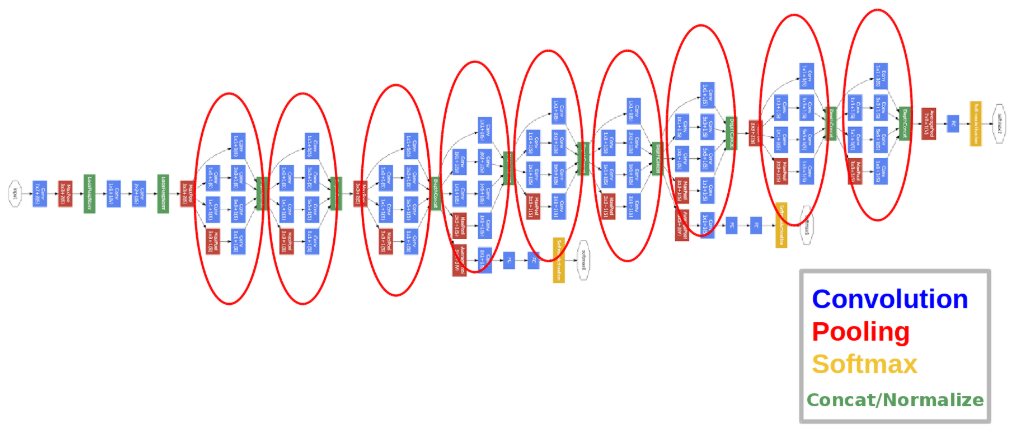
\includegraphics[page={1},width=0.47\textwidth]{./etc/googlenet.PNG}}
		\quad
		{\includegraphics[page={2},width=0.47\textwidth]{./etc/inception_module.PNG}}
		\caption{Inception-v1}
		\label{v1}
	\end{figure}
\end{frame}


\section{Inception-v2/v3}
\begin{frame}{Inception-v2/v3}
	\begin{itemize}
		\item Inception-v2\cite{v2_v3} was created to improve the performance of Inception-v1.
		\item And Inception-v3\cite{v2_v3} is an optimized model by adjusting detailed options based on the Inception-v2 structure.
	\end{itemize}
	\vspace{10pt}
	\begin{figure}[h]		
		\centering
		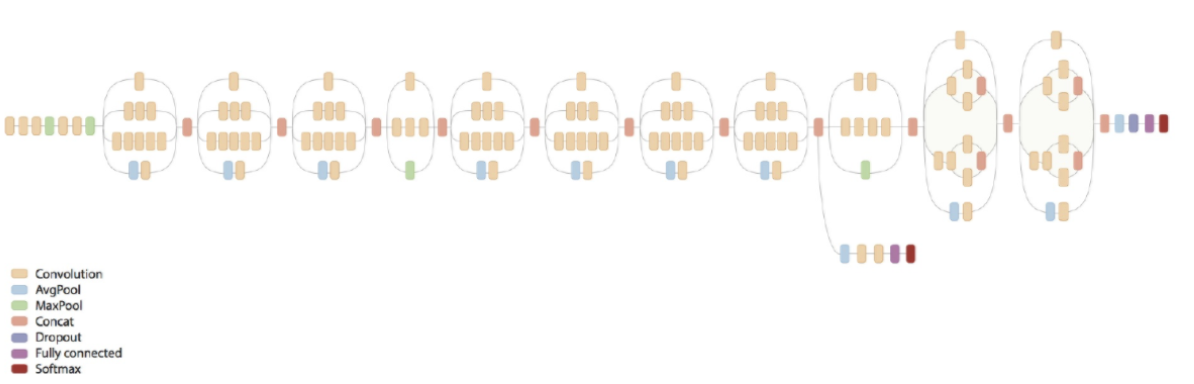
\includegraphics[scale=0.45]{./v2_v3/inception_v2.PNG}
		\caption{Inception-v2 Structure}
		\label{inceptionv2}
	\end{figure}
\end{frame}


\begin{frame}{Inception-v2/v3}
	\begin{itemize}
		\item Inception-v2/v3 have the following characteristics roughly :
		\begin{enumerate}
			\item First auxiliary classifiers is deleted.
			\item Using only $3 \times 3$ filter. (Fig.~\ref{orifactor})
			\item Factorization using asymmetric convolution. (Fig.~\ref{asymconv})
			\item Efficient grid reduction. (Fig.~\ref{poolinception2})
		\end{enumerate}
		\item In addition, Inception-v2/v3 have its own criteria for calculating the number of filters in each stage, such as GoogLeNet.
	\end{itemize}
\end{frame}


\begin{frame}{Inception-v2/v3}
	\begin{itemize}
		\item Using only $3 \times 3$ filter means that :
	\end{itemize}
	\vspace{7pt}
	\begin{figure}[h]		
		\centering
		\subfloat[Original Inception]
		{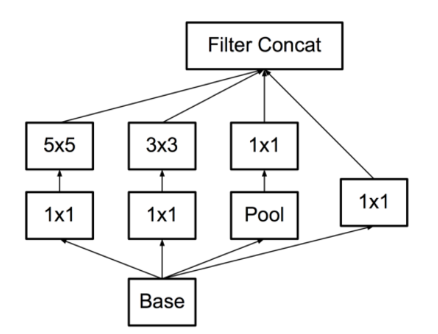
\includegraphics[page={1},width=0.45\textwidth]{./v2_v3/v2_ori.PNG}}
		\quad
		\subfloat[Imporved Inception]
		{\includegraphics[page={2},width=0.45\textwidth]{./v2_v3/v2_factor.PNG}}
		\caption{Using only $3 \times 3$ Filter}
		\label{orifactor}
	\end{figure}
\end{frame}


\begin{frame}{Inception-v2/v3}
	\begin{itemize}
		\item Also, factorization using asymmetric convolution means that :
	\end{itemize}
	\vspace{7pt}
	\begin{figure}[h]		
		\centering
		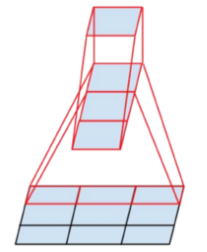
\includegraphics[scale=0.75]{./v2_v3/asym_conv.PNG}
		\caption{Asymmetric Convolution}
		\label{asymconv}
	\end{figure}
\end{frame}


\begin{frame}{Inception-v2/v3}
	\begin{itemize}
		\item And last, efficient grid reduction means that :
		\begin{enumerate}
			\item In general, if we reduce the input size using convolution operation, then increase the filter size for the purpose of trade-off.
			\item Therefore, the order of convolution and pooling is a major concern when they produce same output size.
			\item If you do pooling first, then 'representational bottleneck' occurs.
			\item Otherwise, the amount of calculation is quadruple. ($2(\frac{d}{2})^2 k^2$ $\rightarrow$ $2d^2 k^2$ , $d=35$,$k=320$ ) 
		\end{enumerate}
		\begin{figure}[h]		
			\centering
			\subfloat[Inception First]
			{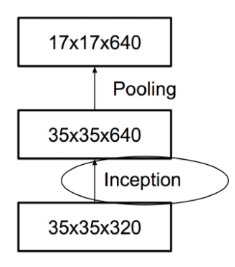
\includegraphics[page={1},width=0.23\textwidth]{./v2_v3/conv_pool.PNG}}
			\quad
			\subfloat[Pooling First]
			{\includegraphics[page={2},width=0.25\textwidth]{./v2_v3/pool_conv.PNG}}
			\caption{Inception \& Pooling Trade-off}
			\label{poolinginception}
		\end{figure}
	\end{itemize}
\end{frame}	
	
	
\begin{frame}{Inception-v2/v3}
	\begin{itemize}
		\item So, consider the picture below(Fig.~\ref{poolinception2}) that compromises these two. 
		\item And this grid reduction will be used after the 'Inception-Block-A/B' operation.
		\item You can check the 'Inception-Block-A/B' in Fig.~\ref{Inception Blocks v2/v3}.
		\vspace{7pt}
		\begin{figure}[h]		
			\centering
			\subfloat[Compromise]
			{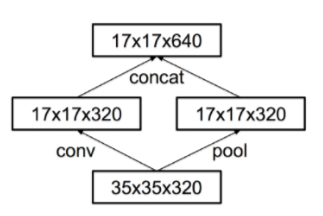
\includegraphics[page={1},width=0.4\textwidth]{./v2_v3/red_sol1.PNG}}
			\quad
			\subfloat[Final Reduction Shape]
			{\includegraphics[page={2},width=0.3\textwidth]{./v2_v3/red_sol2.PNG}}
			\caption{Grid Reduction}
			\label{poolinception2}
		\end{figure}
	\end{itemize}
\end{frame}


\begin{frame}{Inception-v2/v3}
	\begin{itemize}
		\item So, the Inception-v2/v3 structure are as follows :
		\vspace{10pt}
	\begin{figure}[h]		
		\centering
		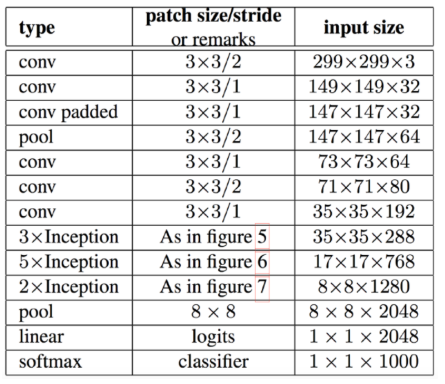
\includegraphics[scale=0.63]{./v2_v3/v2_summary.PNG}
		\caption{Inception-v2/v3 Summary}
		\label{inceptionv2summary}
	\end{figure}
		\item "figure 5,6,7" in Fig.~\ref{inceptionv2summary} are on the next slide.
	\end{itemize}
\end{frame}


\begin{frame}{Inception-v2/v3}
	\begin{itemize}
		\item Each Inception Block-A,B,C has the following form :
		\vspace{3pt}
		\begin{figure}[h]		
			\centering
			\subfloat[Inception-A]
			{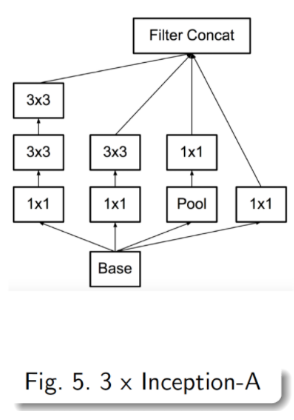
\includegraphics[page={1},width=0.24\textwidth]{./v2_v3/v2_a.PNG}}
			\quad
			\subfloat[Inception-B]
			{\includegraphics[page={2},width=0.24\textwidth]{./v2_v3/v2_b.PNG}}
			\quad
			\subfloat[Inception-C]
			{\includegraphics[page={3},width=0.32\textwidth]{./v2_v3/v2_c.PNG}}
			\caption{Inception Blocks in v2/v3}
			\label{Inception Blocks v2/v3}
		\end{figure}
	\end{itemize}
\end{frame}


\begin{frame}{Inception-v2/v3}
	\begin{itemize}
		\item As Inception-v2 changed to Inception-v3, the following contents were corrected :
		\vspace{7pt}
		\begin{enumerate}
			\item Momentum $\rightarrow$ RMSProp.
			\vspace{4pt}
			\item Label Smoothing Regularization(LSR) : The main purpose of the LSR is to prevent the difference between the largest logit and others. (probability bias prevention)
			\vspace{4pt}
			\item BN in auxiliary classifier : the fully connected layer of the auxiliary classifier is also batch-normalized, not just the convolutions.
		\end{enumerate}
	\end{itemize}
\end{frame}


\section{Inception: -v4 , -ResNet-v1, -ResNet-v2}
\begin{frame}{Advanced Inception}
	\begin{itemize}
		\item Inception-v4, Inception-ResNet-v1 and Inception-ResNet-v2 were published in the same paper\cite{v4etc}.
		\item And Inception-v4, Inception-ResNet-v1, Inception-ResNet-v2 are an improved model of Inception-v3, Inception-v3(with ResNet), Inception-v4 respectively.
		\item As tensorflow\cite{tensorflow} was developed in 2015, it became possible to develop Inception models by removing limitations.
	\end{itemize}
\end{frame}


\begin{frame}{Inception-v4}
	\begin{itemize}
		\item Let's see the Inception-v4.
		\item Inception-v4 structure is as follows :
	\end{itemize}
	\vspace{7pt}
	\begin{figure}[h]		
		\centering
		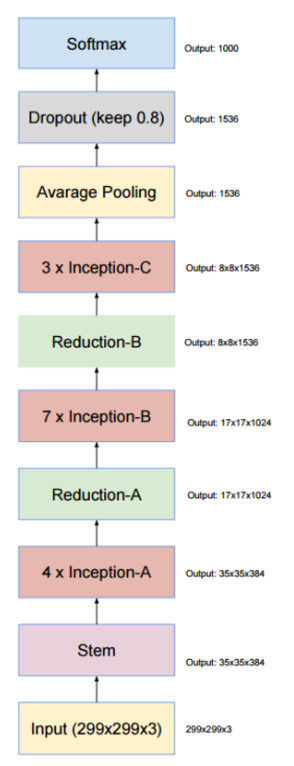
\includegraphics[scale=0.37]{./v4/inception_v4.PNG}
		\caption{Inception-v4 Structure}
		\label{inceptionv4}
	\end{figure}
\end{frame}


\begin{frame}{Inception-v4}
	\begin{itemize}
		\item Inception-v4 is a model in which the structure of Stem, Inception, and Reduction Block is slightly modified in Inception-v3.
		\item Furthermore, auxilary classifier part is all deleted in Inception-v4.
		\item Stem, Inception, Reduction Block are presented in the next slide.
	\end{itemize}
\end{frame}


\begin{frame}{Inception-v4}
	\begin{itemize}
		\item Stem Block in Inception-v4 has the following form :
		\vspace{7pt}
		\begin{figure}[h]		
			\centering
			\includegraphics[scale=0.37]{./v4/stem.PNG}
			\caption{Stem Block}
			\label{stem}
		\end{figure}
	\end{itemize}
\end{frame}


\begin{frame}{Inception-v4}
	\begin{itemize}
		\item Each Inception Block-A,B,C in Inception-v4 has the following form :
		\vspace{10pt}
		\begin{figure}[h]		
			\centering
			\subfloat[Inception-A]
			{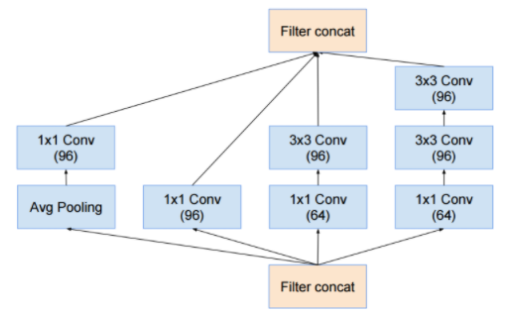
\includegraphics[page={1},width=0.29\textwidth]{./v4/v4_a.PNG}}
			\quad
			\subfloat[Inception-B]
			{\includegraphics[page={2},width=0.29\textwidth]{./v4/v4_b.PNG}}
			\quad
			\subfloat[Inception-C]
			{\includegraphics[page={3},width=0.29\textwidth]{./v4/v4_c.PNG}}
			\caption{Inception Blocks in v4}
			\label{Inception Blocks v4}
		\end{figure}
	\end{itemize}
\end{frame}


\begin{frame}{Inception-v4}
	\begin{itemize}
		\item Each Reduction block-A,B in Inception-v4 has the following form :
		\vspace{10pt}
		\begin{figure}[h]		
			\centering
			\subfloat[Reduction-A]
			{\includegraphics[page={1},width=0.4\textwidth]{./v4/red_a.PNG}}
			\quad
			\subfloat[Reduction-B]
			{\includegraphics[page={2},width=0.38\textwidth]{./v4/red_b.PNG}}
			\caption{Reduction Blocks in v4}
			\label{Reduction Blocks v4}
		\end{figure}
	\end{itemize}
\end{frame}


\begin{frame}{Inception-v4}
	\begin{itemize}
		\item k, l, m, n corresponding to Reducion-A(Fig~\ref{Reduction Blocks v4}) follows the values in the picture below :
		\vspace{13pt}
		\begin{figure}[h]		
			\centering
			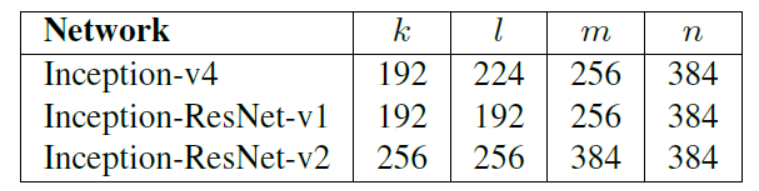
\includegraphics[scale=0.4]{./v4/klmn.PNG}
			\caption{k,l,m,n in Reduction-A}
			\label{klmn}
		\end{figure}
	\end{itemize}
\end{frame}


\begin{frame}{Inception-ResNet-v1/v2}
	\begin{itemize}
		\item Now we consider the model, Inception-ResNet-v1/v2.
		\item Inception-ResNet-v1/v2 has only partially changed in the structure of Inception-v3/v4.
		\item One particular thing is that scaling of the residuals was considered.
	\end{itemize}
\end{frame}


\begin{frame}{Inception-ResNet-v1}
	\begin{itemize}
		\item Let's see the Inception-Resnet-v1.
		\item Inception-ResNet-v1 structure is as follows :
		\vspace{7pt}
		\begin{figure}[h]		
			\centering
			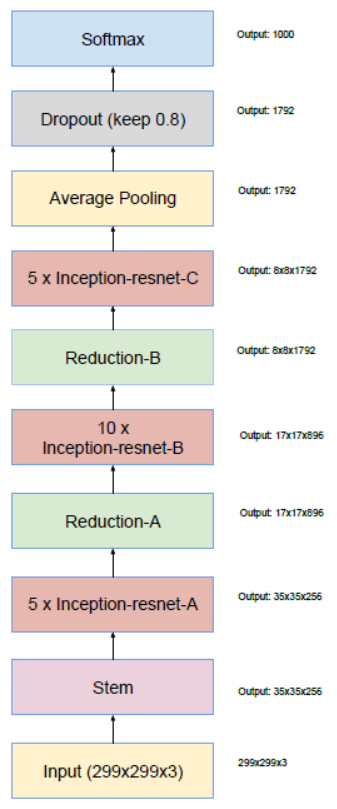
\includegraphics[scale=0.3]{./in_res_v1/incep_res_str.PNG}
			\caption{Inception-ResNet-v1 Structure}
			\label{InceptionResNetv1}
		\end{figure}
	\end{itemize}
\end{frame}


\begin{frame}{Inception-ResNet-v1}
	\begin{itemize}
		\item Stem Block in Inception-ResNet-v1 has the following form :
		\vspace{7pt}
		\begin{figure}[h]		
			\centering
			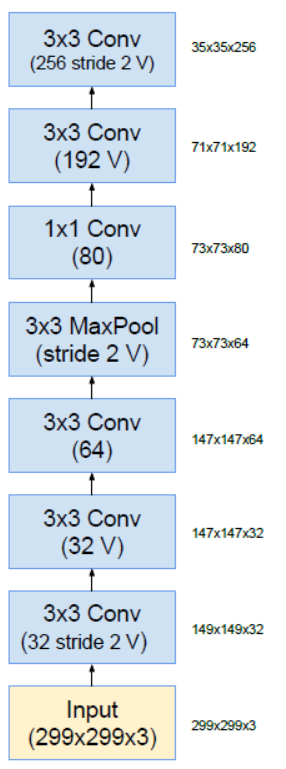
\includegraphics[scale=0.33]{./in_res_v1/stem.PNG}
			\caption{Stem Block}
			\label{steminresv1}
		\end{figure}
		\item It is same as Inception-v3.
	\end{itemize}
\end{frame}


\begin{frame}{Inception-ResNet-v1}
	\begin{itemize}
		\item Each Inception Block-A,B,C in Inception-ResNet-v1 has the following form :
		\vspace{10pt}
		\begin{figure}[h]		
			\centering
			\subfloat[Inception-A]
			{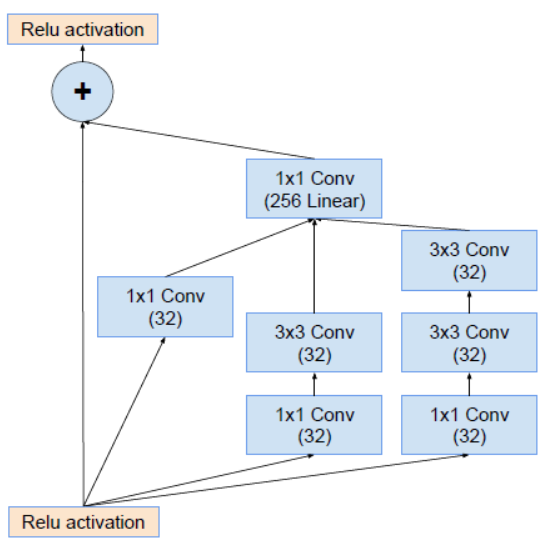
\includegraphics[page={1},width=0.33\textwidth]{./in_res_v1/a.PNG}}
			\quad
			\subfloat[Inception-B]
			{\includegraphics[page={2},width=0.27\textwidth]{./in_res_v1/b.PNG}}
			\quad
			\subfloat[Inception-C]
			{\includegraphics[page={3},width=0.27\textwidth]{./in_res_v1/c.PNG}}
			\caption{Inception-ResNet Blocks in v1}
			\label{Inception-ResNet Blocks v1}
		\end{figure}
	\end{itemize}
\end{frame}


\begin{frame}{Inception-ResNet-v1}
	\begin{itemize}
		\item Each Reduction Block-A,B in Inception-ResNet-v1 has the following form :
		\vspace{5pt}
		\begin{figure}[h]		
			\centering
			\subfloat[Reduction-A]
			{\includegraphics[page={1},width=0.4\textwidth]{./in_res_v1/red_a.PNG}}
			\quad
			\subfloat[Reduction-B]
			{\includegraphics[page={2},width=0.4\textwidth]{./in_res_v1/red_b.PNG}}
			\caption{Reduction Blocks in Inception-ResNet-v1}
			\label{Reduction Blocks v1}
		\end{figure}
		\vspace{5pt}
		\item k,l,m,n in Reduction Block-A are in Fig~\ref{klmn}.
	\end{itemize}
\end{frame}


\begin{frame}{Inception-ResNet-v2}
	\begin{itemize}
		\item Let's see the Inception-Resnet-v2.
		\item Inception-ResNet-v2 structure is as follows :
		\vspace{7pt}
		\begin{figure}[h]		
			\centering
			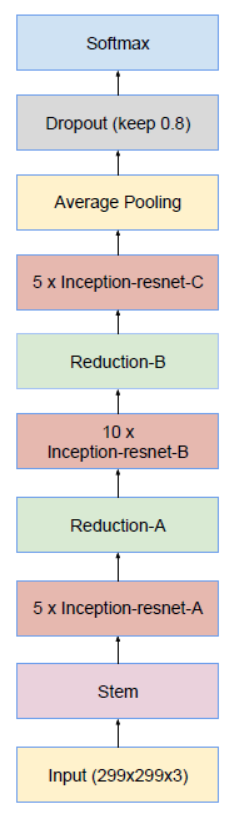
\includegraphics[scale=0.28]{./in_res_v2/str.PNG}
			\caption{Inception-ResNet-v2 Structure}
			\label{InceptionResNetv2}
		\end{figure}
		\item This structure is same as Inception-ResNet-v1.
	\end{itemize}
\end{frame}


\begin{frame}{Inception-ResNet-v2}
	\begin{itemize}
		\item Stem Block in Inception-ResNet-v2 has the following form :
		\vspace{7pt}
		\begin{figure}[h]		
			\centering
			\includegraphics[scale=0.33]{./in_res_v2/stem.PNG}
			\caption{Stem Block}
			\label{steminresv2}
		\end{figure}
		\item It is same as Inception-v4.
	\end{itemize}
\end{frame}


\begin{frame}{Inception-ResNet-v2}
	\begin{itemize}
		\item Each Inception Block-A,B,C in Inception-ResNet-v2 has the following form :
		\vspace{10pt}
		\begin{figure}[h]		
			\centering
			\subfloat[Inception-A]
			{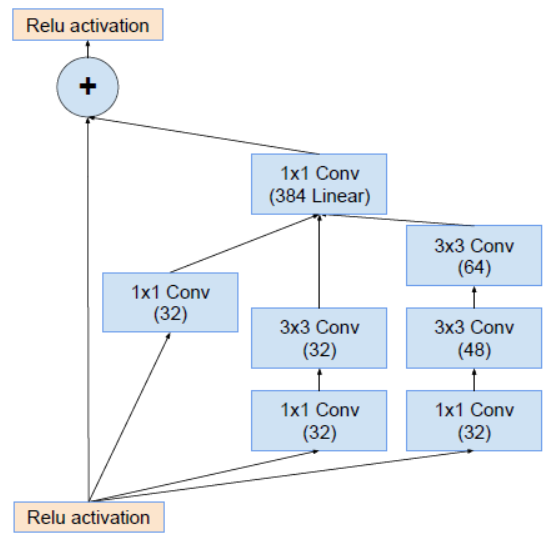
\includegraphics[page={1},width=0.33\textwidth]{./in_res_v2/a.PNG}}
			\quad
			\subfloat[Inception-B]
			{\includegraphics[page={2},width=0.27\textwidth]{./in_res_v2/b.PNG}}
			\quad
			\subfloat[Inception-C]
			{\includegraphics[page={3},width=0.27\textwidth]{./in_res_v2/c.PNG}}
			\caption{Inception-ResNet Blocks in v2}
			\label{Inception-ResNet Blocks v2}
		\end{figure}
	\end{itemize}
\end{frame}


\begin{frame}{Inception-ResNet-v2}
	\begin{itemize}
		\item Each Reduction Block-A,B in Inception-ResNet-v2 has the following form :
		\vspace{5pt}
		\begin{figure}[h]		
			\centering
			\subfloat[Reduction-A]
			{\includegraphics[page={1},width=0.37\textwidth]{./in_res_v2/red_a.PNG}}
			\quad
			\subfloat[Reduction-B]
			{\includegraphics[page={2},width=0.4\textwidth]{./in_res_v2/red_b.PNG}}
			\caption{Reduction Blocks in Inception-ResNet-v2}
			\label{Reduction Blocks v2}
		\end{figure}
		\vspace{5pt}
		\item k,l,m,n in Reduction Block-A are in Fig~\ref{klmn}.
	\end{itemize}
\end{frame}


\begin{frame}{Inception-ResNet-v1/v2 : Scaling of the Residuals }
	\begin{itemize}
		\item And last, if the number of filters exceeded 1000, the residual variants started to exhibit instabilities and the network just “died” early in the training, meaning that the last layer before the average pooling started to produce only zeros after a few tens of thousands of iterations.
		\item This could not be prevented, either by lowering the learning rate, or by
		adding an extra batch-normalization to this layer.
		\item In general we picked some scaling factors between 0.1 and 0.3 to scale the residuals before their being added to the accumulated layer activations.
		\item Even where the scaling was not strictly necessary, it never
		seemed to harmed the final accuracy, but it helped to stabilize
		the training.
	\end{itemize}
\end{frame}


\begin{frame}{Inception-ResNet-v1/v2 : Scaling of the Residuals }
	\begin{itemize}
		\item And this can be usually solved by giving a linear activation function.
		\item Note that only residual terms are assigned a scale between 0.1 and 0.3.
		\vspace{7pt}
		\begin{figure}[h]		
			\centering
			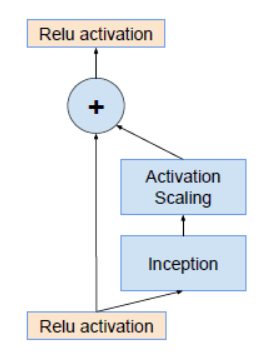
\includegraphics[scale=0.7]{./in_res_v2/scaling.PNG}
			\caption{Scaling of the Residuals}
			\label{scaling}
		\end{figure}
	\end{itemize}
\end{frame}


\section{Reference}
\begin{frame}[allowframebreaks]{Reference}
	\bibliography{references}
\end{frame}

\end{document}
